To test if 
the LSTM layer could be replaced by 
another way of aggregating the convolutional layer outputs, three networks were constructed without any LSTM layer.

One of them, ``CM'' uses a stride of one and aggregates the results using a big max pooling layer.

Another one, ``CCM'' uses the same strategy, but includes another convolutional layer before the max pooling.

The last one, ``CD'', uses a bigger input window of 64 units, but with a smaller stride of 8 units. The output layer is a fully connected layer.

The results are shown in table \ref{tab:carvingnolstm}. The ``CL'' network is included for comparison.
These three networks produced similar results, but they are not as good as the ``CL'' network, as can be seen in figure
\ref{fig:nolstm}.


\begin{table}[!ht]
    \centering
    \caption{No LSTM}
    \label{tab:carvingnolstm}
\begin{tabular}{r|r|r|r|r|r|r}
\hline
Name & Parameters & Blocks & Epochs & Time & Training          & Validation          \\       
     &            &        &        &         &          accuracy &            accuracy \\ \hline\hline

CL & 24663  & all & 150 & 8m38s  & 0.813 & 0.783 \\ \hline
CM  & 24579   & all & 37 & 10m08s & 0.79  & 0.765 \\ \hline
CCM & 24600   & all & 36 & 10m13s & 0.764 & 0.732 \\ \hline
CD  & 1059587 & all & 47 & 10m11s & 0.745 & 0.739 \\ \hline
\end{tabular}
\end{table}

\begin{figure}[htb!]
\centering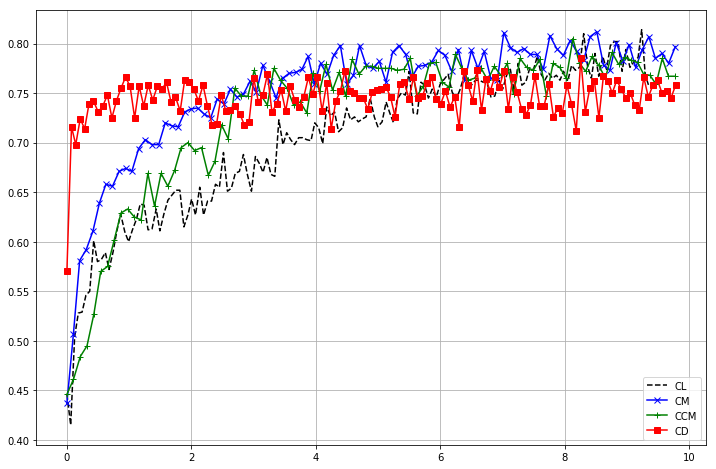
\includegraphics[width=0.65\textwidth]{content/nolstm.png}
\caption{\label{fig:nolstm}No LSTM}%
\end{figure}
\todo[inline]{legenda}

